%%%%%%%%%%%%%%%%%%%%%%%%%%%%%%%%%%%%%%%%%%%%%%%%%%%%%%%%%%%%%%%%%%%%%%%%%%%%%%%%
%                                                                              %
% neural network_1                                                             %
%                                                                              %
% version: 2018-12-05T1836Z                                                    %
%                                                                              %
% Will Breaden Madden                                                          %
%                                                                              %
%%%%%%%%%%%%%%%%%%%%%%%%%%%%%%%%%%%%%%%%%%%%%%%%%%%%%%%%%%%%%%%%%%%%%%%%%%%%%%%%
%                                                                              %
% DESCRIPTION                                                                  %
%                                                                              %
% This program produces a neural network diagram.                              %
%                                                                              %
%%%%%%%%%%%%%%%%%%%%%%%%%%%%%%%%%%%%%%%%%%%%%%%%%%%%%%%%%%%%%%%%%%%%%%%%%%%%%%%%
%                                                                              %
% LICENCE INFORMATION                                                          %
%                                                                              %
% This program produces a document.                                            %
%                                                                              %
% copyright (C) 2015 William Breaden Madden                                    %
%                                                                              %
% This software is released under the terms of the GNU General Public License  %
% version 3 (GPLv3).                                                           %
%                                                                              %
% This program is free software: you can redistribute it and/or modify it      %
% under the terms of the GNU General Public License as published by the Free   %
% Software Foundation, either version 3 of the License, or (at your option)    %
% any later version.                                                           %
%                                                                              %
% This program is distributed in the hope that it will be useful, but WITHOUT  %
% ANY WARRANTY; without even the implied warranty of MERCHANTABILITY or        %
% FITNESS FOR A PARTICULAR PURPOSE.  See the GNU General Public License for    %
% more details.                                                                %
%                                                                              %
% For a copy of the GNU General Public License, see                            %
% <http://www.gnu.org/licenses/>.                                              %
%                                                                              %
%%%%%%%%%%%%%%%%%%%%%%%%%%%%%%%%%%%%%%%%%%%%%%%%%%%%%%%%%%%%%%%%%%%%%%%%%%%%%%%%

\documentclass[border=0.125cm]{standalone}
\usepackage{tikz}
\usetikzlibrary{positioning}
\begin{document}

\tikzset{%
  every neuron/.style={
    circle,
    draw,
    minimum size=1cm
  },
  neuron missing/.style={
    draw=none, 
    scale=4,
    text height=0.333cm,
    execute at begin node=\color{black}${\vdots}$
  },
}

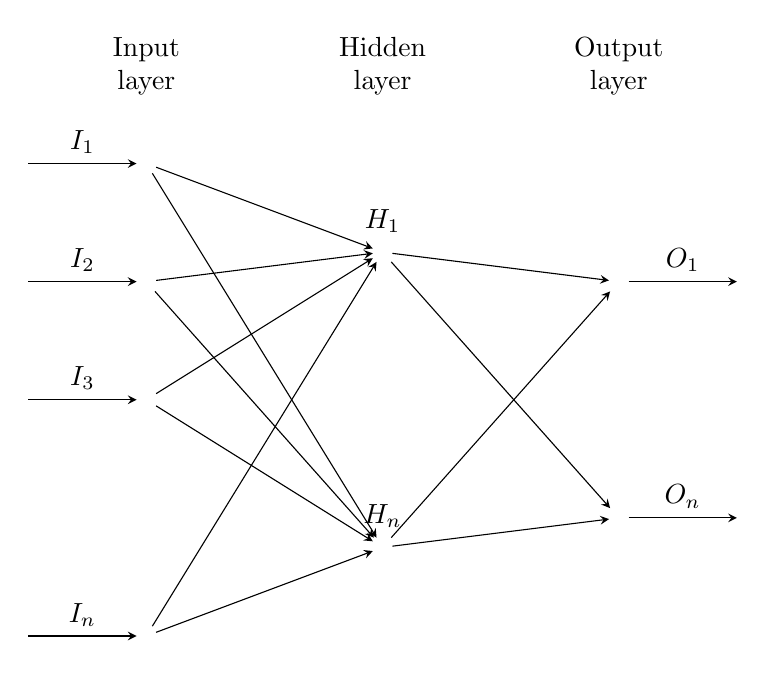
\begin{tikzpicture}[x=1.5cm, y=1.5cm, >=stealth]

\foreach \m/\l [count=\y] in {1, 2, 3, missing, 4}
    \node [every neuron/.try, neuron \m/.try] (input-\m) at (0, 2.5-\y) {};

\foreach \m [count=\y] in {1, missing, 2}
    \node [every neuron/.try, neuron \m/.try ] (hidden-\m) at (2, 2-\y*1.25) {};

\foreach \m [count=\y] in {1, missing, 2}
    \node [every neuron/.try, neuron \m/.try ] (output-\m) at (4, 1.5-\y) {};

\foreach \l [count=\i] in {1, 2, 3, n}
    \draw [<-] (input-\i) -- ++(-1, 0)
        node [above, midway] {${I_\l}$};

\foreach \l [count=\i] in {1, n}
    \node [above] at (hidden-\i.north) {${H_\l}$};

\foreach \l [count=\i] in {1, n}
    \draw [->] (output-\i) -- ++(1, 0)
        node [above, midway] {${O_\l}$};

\foreach \i in {1, ..., 4}
    \foreach \j in {1, ..., 2}
        \draw [->] (input-\i) -- (hidden-\j);

\foreach \i in {1, ..., 2}
    \foreach \j in {1, ..., 2}
        \draw [->] (hidden-\i) -- (output-\j);

\foreach \l [count=\x from 0] in {Input\\layer, Hidden\\layer, Output\\layer}
    \node [align=center, above] at (\x*2, 2) {\l};

\end{tikzpicture}

\end{document}
